%%%%%%%%%%%%%%%%%%%%%%%%%%%%%%%%%%%%%%%%%%%%%%%%%%%%%%%%%%%%%%%%%%%%%%%%%%%%%%%%
% Template for USENIX papers.
%
% History:
%
% - TEMPLATE for Usenix papers, specifically to meet requirements of
%   USENIX '05. originally a template for producing IEEE-format
%   articles using LaTeX. written by Matthew Ward, CS Department,
%   Worcester Polytechnic Institute. adapted by David Beazley for his
%   excellent SWIG paper in Proceedings, Tcl 96. turned into a
%   smartass generic template by De Clarke, with thanks to both the
%   above pioneers. Use at your own risk. Complaints to /dev/null.
%   Make it two column with no page numbering, default is 10 point.
%
% - Munged by Fred Douglis <douglis@research.att.com> 10/97 to
%   separate the .sty file from the LaTeX source template, so that
%   people can more easily include the .sty file into an existing
%   document. Also changed to more closely follow the style guidelines
%   as represented by the Word sample file.
%
% - Note that since 2010, USENIX does not require endnotes. If you
%   want foot of page notes, don't include the endnotes package in the
%   usepackage command, below.
% - This version uses the latex2e styles, not the very ancient 2.09
%   stuff.
%
% - Updated July 2018: Text block size changed from 6.5" to 7"
%
% - Updated Dec 2018 for ATC'19:
%
%   * Revised text to pass HotCRP's auto-formatting check, with
%     hotcrp.settings.submission_form.body_font_size=10pt, and
%     hotcrp.settings.submission_form.line_height=12pt
%
%   * Switched from \endnote-s to \footnote-s to match Usenix's policy.
%
%   * \section* => \begin{abstract} ... \end{abstract}
%
%   * Make template self-contained in terms of bibtex entires, to allow
%     this file to be compiled. (And changing refs style to 'plain'.)
%
%   * Make template self-contained in terms of figures, to
%     allow this file to be compiled. 
%
%   * Added packages for hyperref, embedding fonts, and improving
%     appearance.
%   
%   * Removed outdated text.
%
%%%%%%%%%%%%%%%%%%%%%%%%%%%%%%%%%%%%%%%%%%%%%%%%%%%%%%%%%%%%%%%%%%%%%%%%%%%%%%%%

\documentclass[letterpaper,twocolumn,10pt]{article}
\usepackage{usenix2019_v3}

% to be able to draw some self-contained figs
\usepackage{tikz}
\usepackage{amsmath}

\usepackage[caption=false]{subfig}

%-------------------------------------------------------------------------------
\begin{document}
%-------------------------------------------------------------------------------

% Macros
\newcommand{\todo}[1]{\textbf{TODO: #1}}
\newcommand{\ccite}[1]{~\cite{#1}}

\renewcommand{\L}{\mathcal{L}}
\renewcommand{\P}{\mathcal{P}}
\renewcommand{\O}{\mathcal{O}}
\newcommand{\R}{\mathcal{R}}
\renewcommand{\r}{\mathit{r}}
\renewcommand{\cap}{\mathit{c}}

%don't want date printed
\date{}

% make title bold and 14 pt font (Latex default is non-bold, 16 pt)
\title{\Large \bf A good title}

%for single author (just remove % characters)
\author{
{\rm Your N.\ Here}\\
Your Institution
\and
{\rm Second Name}\\
Second Institution
% copy the following lines to add more authors
% \and
% {\rm Name}\\
%Name Institution
} % end author

\maketitle

%-------------------------------------------------------------------------------
\begin{abstract}
%-------------------------------------------------------------------------------
Abstract
\end{abstract}


%-------------------------------------------------------------------------------
\section{Introduction}
%-------------------------------------------------------------------------------

A paragraph of text goes here.

%-------------------------------------------------------------------------------
\section{Evaluation}
%-------------------------------------------------------------------------------

We used 233 topologies from the Topology Zoo\ccite{topologyzoo}.
We modified these topologies to remove part of the graphs that lack link redundancy,\dots trees.
The resulting topologies have only routers with at least two links.
Communication between routers in a tree can only use a single path.
Such trees cannot see any improvement from using Segment Routing.
Moreover, such trees are likely artifacts of the topology collection
because they cannot preserve connectivity even with a single link failure.
Figure \ref{fig:topo:routers} and \ref{fig:topo:links} shows the CDF
of the number of routers and links in the resulting topologies.
Figure \ref{fig:topo:degree} shows the distributions of routers percentage with a given number
of attached links.

\begin{figure*}
	\centering
	\subfloat[Number of routers\label{fig:topo:routers}]{%
		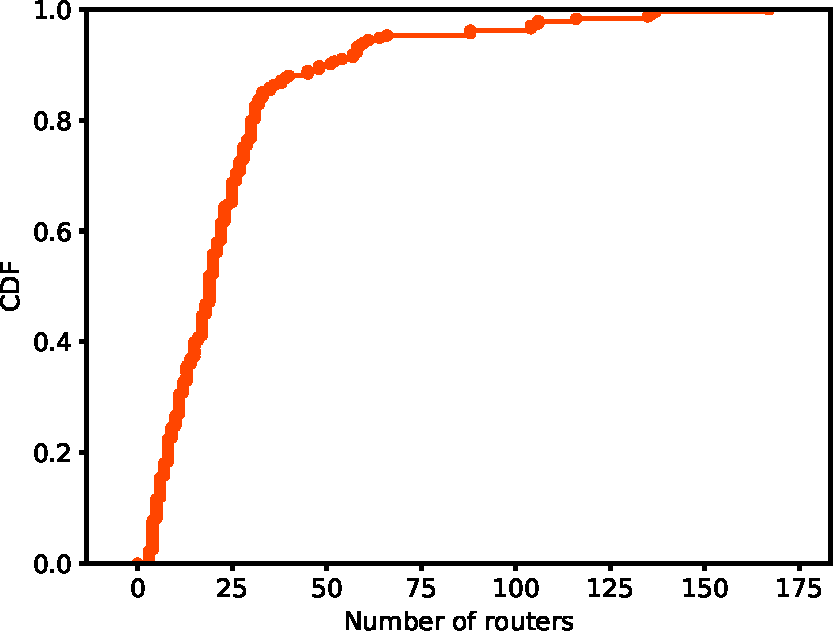
\includegraphics[width=0.3\textwidth]{figs/solver_number_routers_cdfs.pdf}
	}
	\subfloat[Number of links\label{fig:topo:links}]{%
		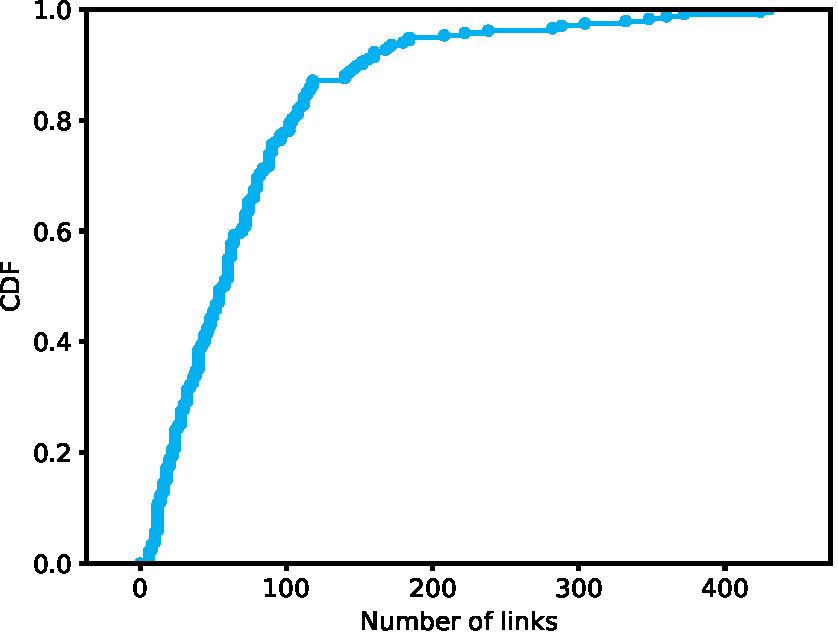
\includegraphics[width=0.3\textwidth]{figs/solver_number_links_cdfs.pdf}
	}
	\subfloat[Out degree of the routers\label{fig:topo:degree}]{%
		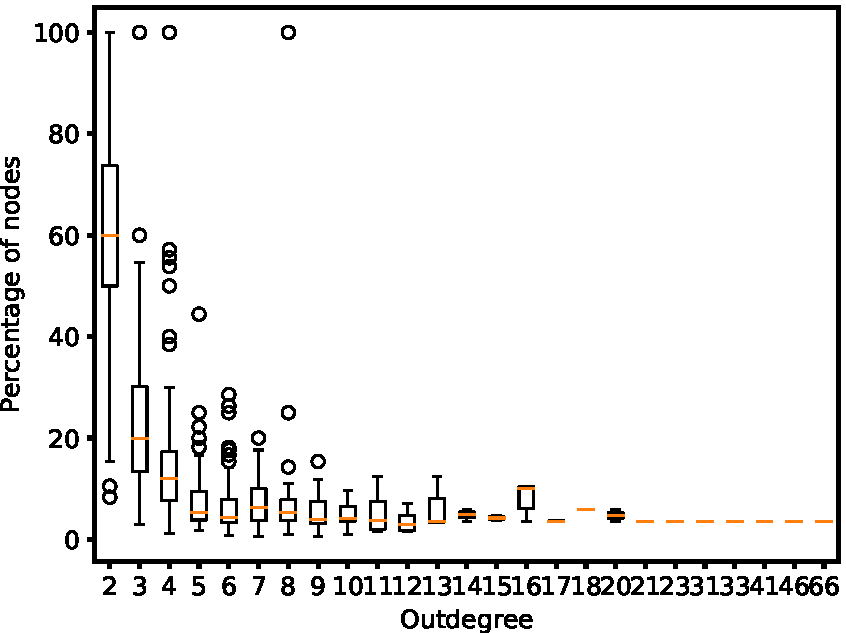
\includegraphics[width=0.303\textwidth]{figs/boxplot_network_outdegree_boxplots.pdf}
	}
	\caption{Features of the evaluation topologies}
	\label{fig:topo}
\end{figure*}

The set of topologies does not include which routers are actually linked to endhosts
and which are core routers. We assume that routers with two links are edge routers
and the others are core routers because they are more connected.

\subsection{Maximum improvement}

This sections evaluation the theoritical improvement of using
multipath transport protocols and Segment Routing on the endhosts
instead of a single path protocol with only shortest paths.

We used a linear programming formulation of the Max Flow problem.
Given a set of paths linking a set of the edge routers, we compute
the maximum amount of traffic that can go through the topology without
exceeding the link capacity.

\begin{equation*}
	\setlength\arraycolsep{0.2pt}
	\begin{smallmatrix}
		\displaystyle maxflow(\P) & & \\
		\displaystyle \max_{f} & \displaystyle \sum_{p \in \P} f_{p} & \\[0.5cm]
		\textrm{s.t.}          & \displaystyle \sum_{p \in \P} \r(l, p) \cdot f_{p} & \displaystyle \leq & \displaystyle \cap(l) & \forall l \in \L
	\end{smallmatrix}
\end{equation*}

$\P$ represents the set of \texttt{sr-paths}, encoded as a list of intermediate routers.
As for IPv6 SR, The real path taken between each intermediate router is the shortest one.
$\r(l, p)$ represents the ratio of flow that goes through a particular link.
This ratio is used to model the ECMP splitting of the traffic.

To model a single-path transport protocol without SR
we insert all the shortest sr-paths between each pair of edge router to $\P$.
We assume that we have a high number of connections for each path
and therefore that hash-based ECMP splits the traffic evenly.
\cite{ecmphashperf} shows that it is not the case in practise.

Multipath transport protocols with SR also uses shortest path routing.
However, they can establish a big number of subflows for each connection
and hope that they will cover all or a portion of the shortest paths.
This hijacks ECMP that sees subflows as indepedent connections.
Flow Bender\ccite{flowbender} and SEMPER\ccite{semper} used this solution to leverage
some of the path diversity of a topology.
We will assume for simplicity that this method works perfectly and that multipath protocols
can always cover all the shortest paths.
We insert a sr-path for each shortest path between each pair of edge routers
instead of giving one sr-path representing all the shortest paths between a given pair. 

Introducing Segment Routing means adding more paths to $\P$.
Note that generating the set of all possible paths is in $\O(|\R|^k)$
with $\R$ being the set of routers and $k$ the maximum number of intermediate nodes.
This is not practicle for big topologies.
Therefore, we reuse the approach of \cite{cg4sr} that iteratively adds relevant paths to the set
until no interesting paths can be added to $\P$.
When it reaches this point, computing the model on this restricted set or on the complete one
gives the same solution.
\todo{Explain how the model is different from infocom, i.e., demands become unbounded or is it too detailed ?}

\textbf{Adding IPv6 SR improves the maximum throughput by \todo{values}\%.}
Figure \ref{fig:maxflow-theory} shows the relative maxfimum flow improvement of using single path or multiple path with Segment Routing. \todo{Add the graph + detailed description of why 1\%, 5\% and 10\% of heavy hitters}

\begin{figure*}
	\centering
	\subfloat[Single path transport protocol\label{fig:fig:maxflow-theory:tcp}]{%
		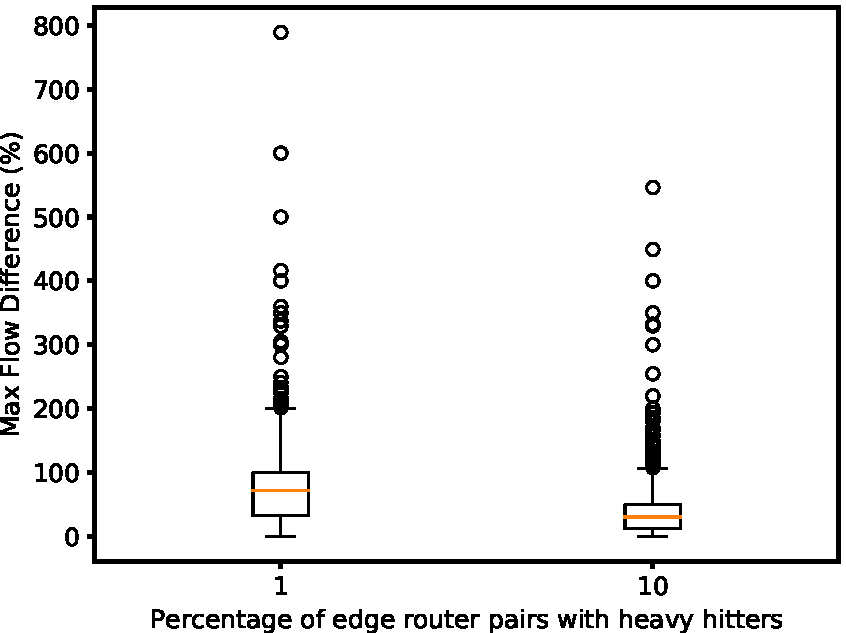
\includegraphics[width=0.4\textwidth]{figs/boxplot_maxflow_diff_accesslinks_2_tcp_segs_ecmp_0_0_boxplots.pdf}
	}
	\subfloat[Multiple path transport protocol\label{fig:fig:maxflow-theory:mptcp}]{%
		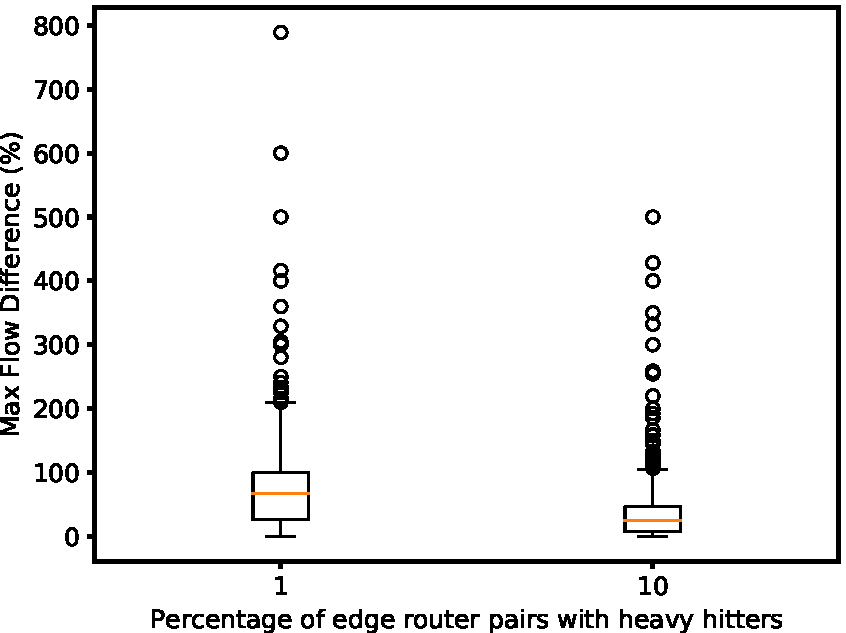
\includegraphics[width=0.4\textwidth]{figs/boxplot_maxflow_diff_accesslinks_2_mptcp_segs_ecmp_0_0_boxplots.pdf}
	}
	\caption{Relative Maxflow improvement of adding IPv6 SR}
	\label{fig:maxflow-theory}
\end{figure*}

%-------------------------------------------------------------------------------
\bibliographystyle{plain}
\bibliography{biblio}

%%%%%%%%%%%%%%%%%%%%%%%%%%%%%%%%%%%%%%%%%%%%%%%%%%%%%%%%%%%%%%%%%%%%%%%%%%%%%%%%
\end{document}
%%%%%%%%%%%%%%%%%%%%%%%%%%%%%%%%%%%%%%%%%%%%%%%%%%%%%%%%%%%%%%%%%%%%%%%%%%%%%%%%

%%  LocalWords:  endnotes includegraphics fread ptr nobj noindent
%%  LocalWords:  pdflatex acks
